% Способ использования БПХ для определения наклона шрифта.

Быстрое преобразование Хафа может быть использовано для определения наклона шрифта. Рассмотрим следующее изображение:
\begin{figure}[!h]
    \centering
    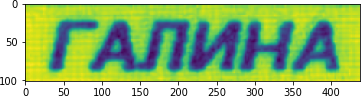
\includegraphics[width=0.7\linewidth]{15_1}
    \caption{Исходное изображение}
\end{figure}

Выделим на изображении границы путем вычитания из изображения его дилатации. Также здесь изображение было отражено относительно вертикальной оси, поскольку шрифт, очевидно, наклонен вправо, а стандартная версия быстрого преобразования Хафа работает с прямыми, наклоненными влево с точки стандартной системы координат изображения.
\begin{figure}[!h]
    \centering
    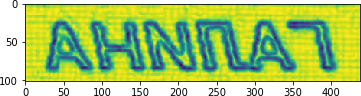
\includegraphics[width=0.7\linewidth]{15_2}
    \caption{Выделенные границы на изображении}
\end{figure}

Применим к полученному изображению БПХ:
\begin{figure}[!h]
    \centering
    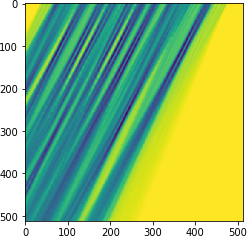
\includegraphics[width=0.35\linewidth]{15_3}
    \caption{Результат применения БПХ к изображению}
\end{figure}

В полученном массиве каждая точка описывает сумму значений по некоторой дискретной прямой, причем $i$-я строка соответствует семейству прямых с определенным наклоном $\theta_i = \arctan\left( \frac{n-1}{i} \right)$. Ясно, что среди всех таких семейств то, которое накладывается на особенности шрифта, будет иметь наибольшую изменчивость: от 0 в промежутках между буквами до высоты строки в случае наложения на <<вертикальный>> элемент буквы. Следовательно, нужно выбрать строку, значения в которой обладают наибольшей дисперсией (или наибольшим стандартным отклонением):
\begin{figure}[!h]
    \centering
    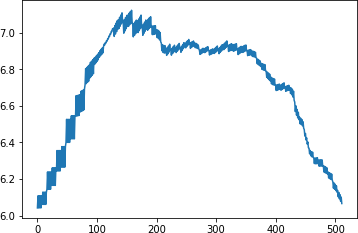
\includegraphics[width=0.5\linewidth]{15_4}
    \caption{График стандартных отклонений строк}
\end{figure}

В данном случае максимальной дисперсией обладает строка $i=158$, описывающая прямые с наклоном $\theta_{158} = \arctan\left( \frac{511}{158} \right) \approx 73^{\circ}$.
\begin{figure}[!h]
    \centering
    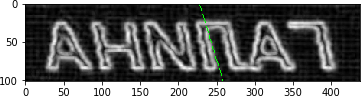
\includegraphics[width=0.5\linewidth]{15_5}
    \caption{Изображение со случайно выбранной прямой из найденного семейства}
\end{figure}
